%\newpage
\chapter{\\The AST to CFG class}
\label{App:SampleEuGENia}
%
\lstinputlisting[language=EOL]{code/sample_gmf.emf}
%
%\lstinputlisting[language=java, breaklines=true]{/Users/thomaswormald/Documents/workspace/all/org.eclipse.epsilon/trunk/plugins/org.eclipse.epsilon.eol.engine/src/org/eclipse/epsilon/eol/parse/ASTtoCFG.java}
%
%%\newpage
%%\chapter{\\Statement Coverage HTML Output Class}
%%\label{App:StatementHTMLOutput}
%%\lstinputlisting[language=java]{code/StatementCoverageToHTML.java}

\chapter{\\Statement Coverage Results}
\label{App:StatementCoverage}

The following pages are the results from statement coverage of the EuGENia source code. The default output is a HTML page. To include this in the appendix the document was printed to a PDF file and then included with this document.

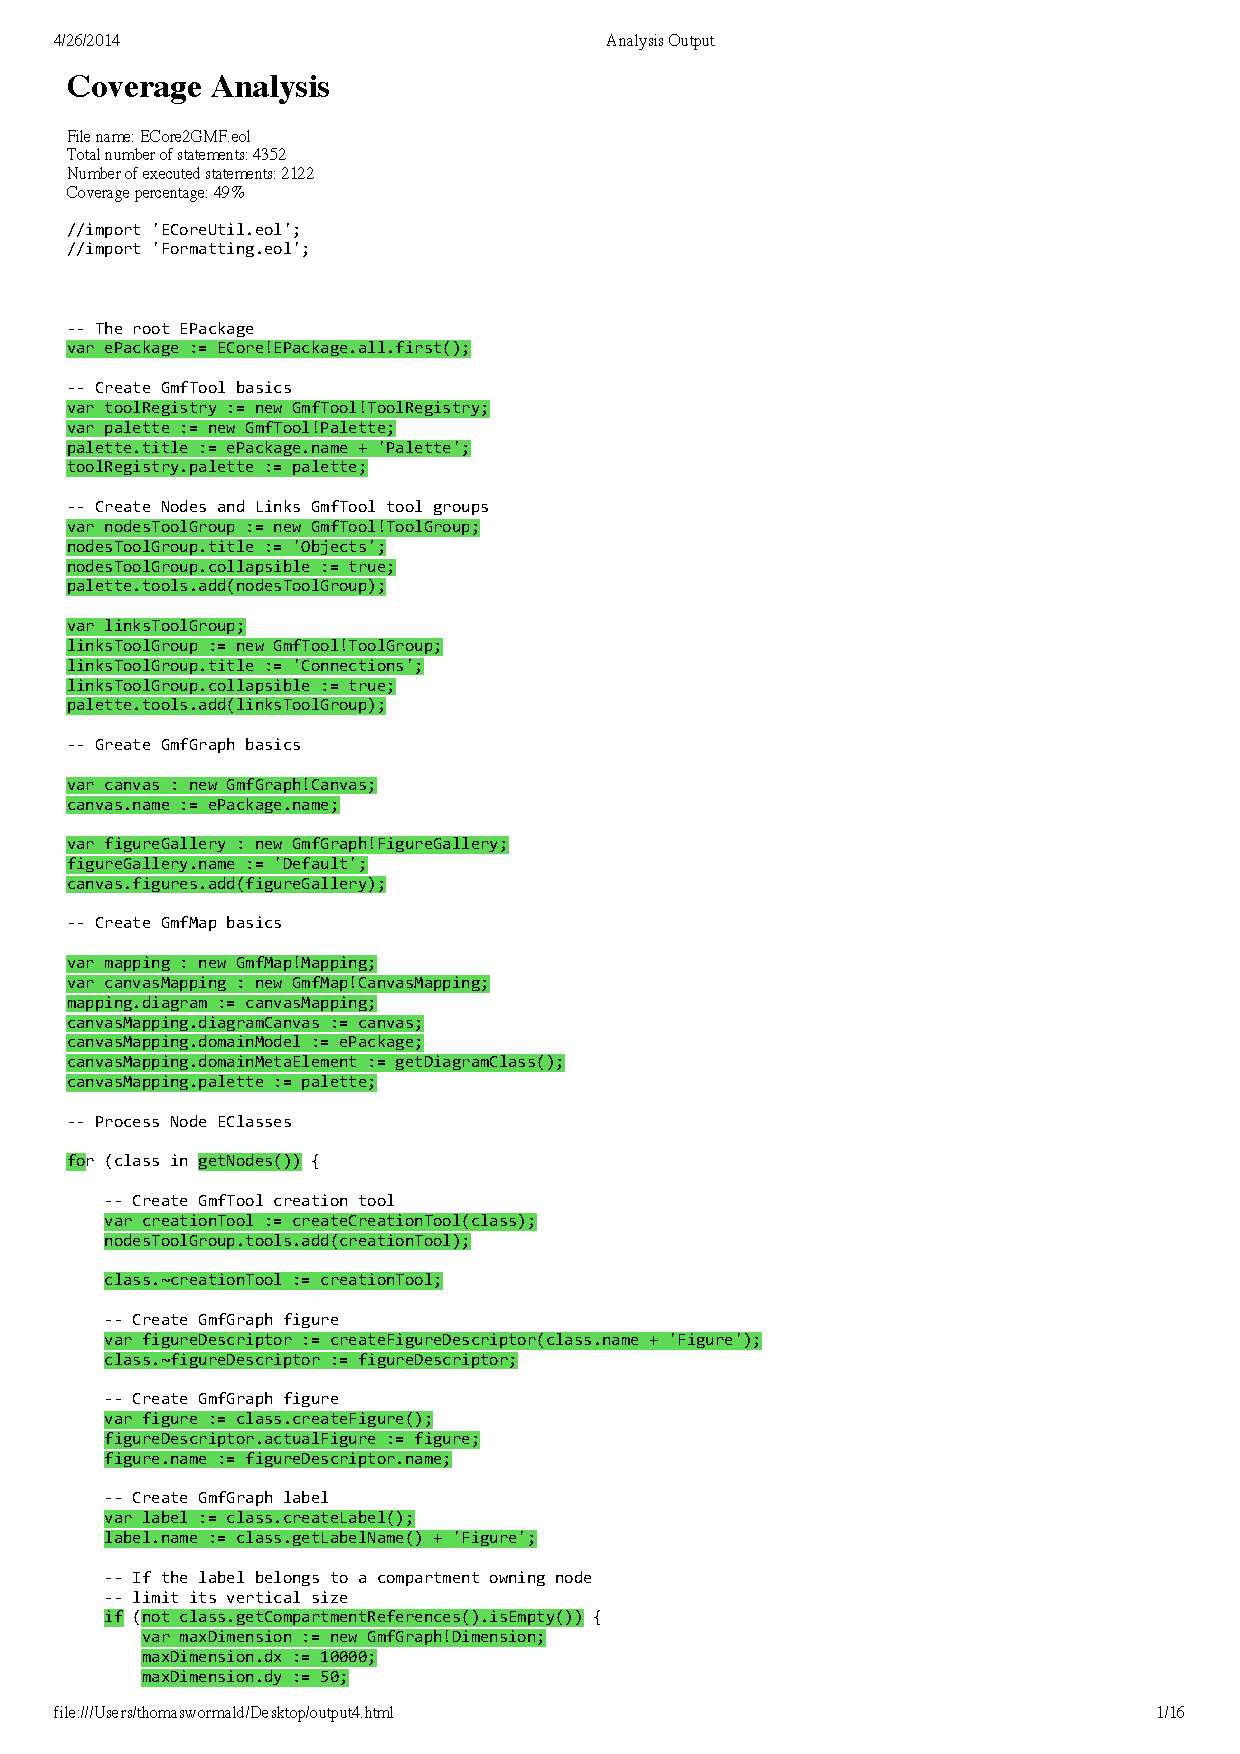
\includepdf[pages={1-16}]{code/statement_coverage.pdf}

\chapter{Path Coverage}

This chapter was what had been documented about path coverage before the decision was made to not include it in the main report. It ends rather abruptly, and does not reflect the state of the code. At the time of writing, the code is a lot more advanced than this chapter implies.

\section{Introduction}

This chapter will detail my implementation of path coverage analysis for EOL. As with the statement coverage and branch coverage chapters, an analysis will be performed, followed by design, implementation, testing and conclusions. This chapter will be more brief than the branch coverage chapter because a lot of the hard work (i.e. the AST to CFG conversion) does not need repeating.

\section{Analysis}

To measure the execution path through a program, every branch that is executed can be recorded as a series of steps. It is not useful to record what is executed between two branches, because that will always be the same. 

Two recorded paths can then be compared by going through each step, and seeing whether the branch taken at each step was the same. There is a slight complexity that must be considered, however. Loops can be executed any number of times, as was discussed in the literature review. I have decided to go with the approach of recording whether a loop was executed zero, or more than zero times. This means that when comparing two paths and one has executed a loop 10 times and the other path has executed it 100 times, these will be considered the same.

Another problem with loops is that they can contain break, breakAll or continue statements which take the control flow of the program outside of the loop, or back to the loop header. Consider the example in Figure \ref{fig:pathCoverageProblem}.
29th august 14
\begin{figure}
\centering
\begin{minipage}{.33\textwidth}
  \centering
  \lstinputlisting[language=EOL]{code/pathcoverageproblem.eol}
\end{minipage}%
\begin{minipage}{.5\textwidth}
  \centering
  \includedot[scale=0.3]{figures/pathloopproblem}
\end{minipage}
\caption{A problematic example}
\label{fig:pathCoverageProblem}
\end{figure}
%http://books.google.co.uk/books?id=qVkgJYh47tEC&pg=PA144&lpg=PA144&dq=path+coverage+loops&source=bl&ots=xwwset1Z33&sig=F6zAK0i7TchDwQOYcvt4FM9wXA0&hl=en&sa=X&ei=ARlVU9uPCs3JOeW6gIAF&ved=0CE8Q6AEwBA#v=onepage&q=path%20coverage%20loops&f=false

This is a difficult problem to solve, and with limited time and space I am going to put the problem to one side. An analysis of the EuGENia source code shows that there are no break or breakAll statements, and there is only a single continue statement, so this should not be a problem. 

\section{Design}

As with the two previous implementations, an execution listener will be implemented. This listener will use much of the same code as the branch listener, because it needs to determine when a branch has been executed. It will not extend the branch listener though, because most of the code is held within one function, and this function needs to be modified, so extending the branch listener would not be useful.

When the branch is to be marked as executed, a the edge that was taken on the graph must be recorded. Because the CFG class doesn't actually contain a list of edge objects that have unique identifiers, recording which edges have been executed is slightly more difficult. As well as storing individual edges, there needs to be a way of storing a collection of executed edges, which will be the path that was taken through the program. 

Two classes will be created then. The first will store the unique ID of the start CFG and the unique ID of the end CFG, which will allow unique identification of an edge. The second class will store a list of the first class, and will implement methods to compare itself to another instance of the same class, allowing for easy comparison of two paths. The comparison method will take into account that we only care whether a loop has been executed zero times or more than zero times.


%\chapter{\\Branch Coverage Results}
%\label{App:BranchCoverage}

%
% ls *.dot | cut -d '.' -f 1 | awk '{printf "\\begin{minipage}[b]{0.5\\textwidth}\n\\centering\n\\includedot[scale=0.3]{./figures/branchgraphs/%s}\nFunction %s\n\\end{minipage}\n", $1, $1}' 


\begin{minipage}[b]{0.5\textwidth}
\centering
\includedot[height=0.8\textheight]{./figures/branchgraphs/createClosedArrow}
Function createClosedArrow
\end{minipage}
\begin{minipage}[b]{0.5\textwidth}
\centering
\includedot[height=0.8\textheight]{./figures/branchgraphs/createColor}
Function createColor
\end{minipage}
\begin{minipage}[b]{0.5\textwidth}
\centering
\includedot[height=0.8\textheight]{./figures/branchgraphs/createCreationTool}
Function createCreationTool
\end{minipage}
\begin{minipage}[b]{0.5\textwidth}
\centering
\includedot[height=0.8\textheight]{./figures/branchgraphs/createDimension}
Function createDimension
\end{minipage}
\begin{minipage}[b]{0.5\textwidth}
\centering
\includedot[height=0.8\textheight]{./figures/branchgraphs/createFigure}
Function createFigure
\end{minipage}
\begin{minipage}[b]{0.5\textwidth}
\centering
\includedot[height=0.8\textheight]{./figures/branchgraphs/createFigureDescriptor}
Function createFigureDescriptor
\end{minipage}
\begin{minipage}[b]{0.5\textwidth}
\centering
\includedot[scale=0.3]{./figures/branchgraphs/createLabel}
Function createLabel
\end{minipage}
\begin{minipage}[b]{0.5\textwidth}
\centering
\includedot[scale=0.3]{./figures/branchgraphs/createPoint}
Function createPoint
\end{minipage}
\begin{minipage}[b]{0.5\textwidth}
\centering
\includedot[height=0.8\textheight]{./figures/branchgraphs/createPolylineDecoration}
Function createPolylineDecoration
\end{minipage}
\begin{minipage}[b]{0.5\textwidth}
\centering
\includedot[height=0.8\textheight]{./figures/branchgraphs/createRefLinkIcon}
Function createRefLinkIcon
\end{minipage}
\begin{minipage}[b]{0.5\textwidth}
\centering
\includedot[height=0.8\textheight]{./figures/branchgraphs/createReferenceCreationTool}
Function createReferenceCreationTool
\end{minipage}
\begin{minipage}[b]{0.5\textwidth}
\centering
\includedot[height=0.8\textheight]{./figures/branchgraphs/createRhomb}
Function createRhomb
\end{minipage}
\begin{minipage}[b]{0.5\textwidth}
\centering
\includedot[height=0.8\textheight]{./figures/branchgraphs/createSquare}
Function createSquare
\end{minipage}
\begin{minipage}[b]{0.5\textwidth}
\centering
\includedot[height=0.8\textheight]{./figures/branchgraphs/createToolImage}
Function createToolImage
\end{minipage}
\begin{minipage}[b]{0.5\textwidth}
\centering
\includedot[height=0.8\textheight]{./figures/branchgraphs/formatConnection}
Function formatConnection
\end{minipage}
\begin{minipage}[b]{0.5\textwidth}
\centering
\includedot[height=0.8\textheight]{./figures/branchgraphs/formatLine}
Function formatLine
\end{minipage}
\begin{minipage}[b]{0.5\textwidth}
\centering
\includedot[height=0.8\textheight]{./figures/branchgraphs/formatNode}
Function formatNode
\end{minipage}
\begin{minipage}[b]{0.5\textwidth}
\centering
\includedot[scale=0.3]{./figures/branchgraphs/getAffixedReferences}
Function getAffixedReferences
\end{minipage}
\begin{minipage}[b]{0.5\textwidth}
\centering
\includedot[scale=0.3]{./figures/branchgraphs/getAllConcreteSubTypes}
Function getAllConcreteSubTypes
\end{minipage}
\begin{minipage}[b]{0.5\textwidth}
\centering
\includedot[scale=0.3]{./figures/branchgraphs/getAllSuitableContainmentReferences}
Function getAllSuitableContainmentReferences
\end{minipage}
\begin{minipage}[b]{0.5\textwidth}
\centering
\includedot[scale=0.3]{./figures/branchgraphs/getAnnotation}
Function getAnnotation
\end{minipage}
\begin{minipage}[b]{0.5\textwidth}
\centering
\includedot[height=0.8\textheight]{./figures/branchgraphs/getAnnotationValue}
Function getAnnotationValue
\end{minipage}
\begin{minipage}[b]{0.5\textwidth}
\centering
\includedot[scale=0.3]{./figures/branchgraphs/getCompartmentReferences}
Function getCompartmentReferences
\end{minipage}
\begin{minipage}[b]{0.5\textwidth}
\centering
\includedot[scale=0.3]{./figures/branchgraphs/getConcreteSubtypes}
Function getConcreteSubtypes
\end{minipage}
\begin{minipage}[b]{0.5\textwidth}
\centering
\includedot[scale=0.3]{./figures/branchgraphs/getContainmentReferences}
Function getContainmentReferences
\end{minipage}
\begin{minipage}[b]{0.5\textwidth}
\centering
\includedot[scale=0.3]{./figures/branchgraphs/getDetail}
Function getDetail
\end{minipage}
\begin{minipage}[b]{0.5\textwidth}
\centering
\includedot[scale=0.3]{./figures/branchgraphs/getDiagramClass}
Function getDiagramClass
\end{minipage}
\begin{minipage}[b]{0.5\textwidth}
\centering
\includedot[scale=0.3]{./figures/branchgraphs/getDiagramContainmentReference}
Function getDiagramContainmentReference
\end{minipage}
\begin{minipage}[b]{0.5\textwidth}
\centering
\includedot[scale=0.3]{./figures/branchgraphs/getDomainMetaElement}
Function getDomainMetaElement
\end{minipage}
\begin{minipage}[b]{0.5\textwidth}
\centering
\includedot[scale=0.3]{./figures/branchgraphs/getFormatOption}
Function getFormatOption
\end{minipage}
\begin{minipage}[b]{0.5\textwidth}
\centering
\includedot[scale=0.3]{./figures/branchgraphs/getLabelAttributes}
Function getLabelAttributes
\end{minipage}
\begin{minipage}[b]{0.5\textwidth}
\centering
\includedot[scale=0.3]{./figures/branchgraphs/getLabelClass}
Function getLabelClass
\end{minipage}
\begin{minipage}[b]{0.5\textwidth}
\centering
\includedot[scale=0.3]{./figures/branchgraphs/getLabelEditPattern}
Function getLabelEditPattern
\end{minipage}
\begin{minipage}[b]{0.5\textwidth}
\centering
\includedot[scale=0.3]{./figures/branchgraphs/getLabelName}
Function getLabelName
\end{minipage}
\begin{minipage}[b]{0.5\textwidth}
\centering
\includedot[scale=0.3]{./figures/branchgraphs/getLabelParser}
Function getLabelParser
\end{minipage}
\begin{minipage}[b]{0.5\textwidth}
\centering
\includedot[scale=0.3]{./figures/branchgraphs/getLabelPattern}
Function getLabelPattern
\end{minipage}
\begin{minipage}[b]{0.5\textwidth}
\centering
\includedot[scale=0.3]{./figures/branchgraphs/getLabelPlacement}
Function getLabelPlacement
\end{minipage}
\begin{minipage}[b]{0.5\textwidth}
\centering
\includedot[scale=0.3]{./figures/branchgraphs/getLabelReadOnly}
Function getLabelReadOnly
\end{minipage}
\begin{minipage}[b]{0.5\textwidth}
\centering
\includedot[scale=0.3]{./figures/branchgraphs/getLabelText}
Function getLabelText
\end{minipage}
\begin{minipage}[b]{0.5\textwidth}
\centering
\includedot[scale=0.3]{./figures/branchgraphs/getLabelViewPattern}
Function getLabelViewPattern
\end{minipage}
\begin{minipage}[b]{0.5\textwidth}
\centering
\includedot[scale=0.3]{./figures/branchgraphs/getLabelledAttributesFor}
Function getLabelledAttributesFor
\end{minipage}
\begin{minipage}[b]{0.5\textwidth}
\centering
\includedot[scale=0.3]{./figures/branchgraphs/getLinkEndFeature}
Function getLinkEndFeature
\end{minipage}
\begin{minipage}[b]{0.5\textwidth}
\centering
\includedot[scale=0.3]{./figures/branchgraphs/getLinkIncoming}
Function getLinkIncoming
\end{minipage}
\begin{minipage}[b]{0.5\textwidth}
\centering
\includedot[scale=0.3]{./figures/branchgraphs/getLinkLabel}
Function getLinkLabel
\end{minipage}
\begin{minipage}[b]{0.5\textwidth}
\centering
\includedot[scale=0.3]{./figures/branchgraphs/getLinkSourceFeature}
Function getLinkSourceFeature
\end{minipage}
\begin{minipage}[b]{0.5\textwidth}
\centering
\includedot[scale=0.3]{./figures/branchgraphs/getLinkTargetFeature}
Function getLinkTargetFeature
\end{minipage}
\begin{minipage}[b]{0.5\textwidth}
\centering
\includedot[scale=0.3]{./figures/branchgraphs/getLinks}
Function getLinks
\end{minipage}
\begin{minipage}[b]{0.5\textwidth}
\centering
\includedot[scale=0.3]{./figures/branchgraphs/getLongName}
Function getLongName
\end{minipage}
\begin{minipage}[b]{0.5\textwidth}
\centering
\includedot[scale=0.3]{./figures/branchgraphs/getNodeSize}
Function getNodeSize
\end{minipage}
\begin{minipage}[b]{0.5\textwidth}
\centering
\includedot[scale=0.3]{./figures/branchgraphs/getNodes}
Function getNodes
\end{minipage}
\begin{minipage}[b]{0.5\textwidth}
\centering
\includedot[scale=0.3]{./figures/branchgraphs/getOneSuitableContainmentReference}
Function getOneSuitableContainmentReference
\end{minipage}
\begin{minipage}[b]{0.5\textwidth}
\centering
\includedot[scale=0.3]{./figures/branchgraphs/getPhantomNodes}
Function getPhantomNodes
\end{minipage}
\begin{minipage}[b]{0.5\textwidth}
\centering
\includedot[scale=0.3]{./figures/branchgraphs/getReadOnly}
Function getReadOnly
\end{minipage}
\begin{minipage}[b]{0.5\textwidth}
\centering
\includedot[scale=0.3]{./figures/branchgraphs/getReferenceLinks}
Function getReferenceLinks
\end{minipage}
\begin{minipage}[b]{0.5\textwidth}
\centering
\includedot[scale=0.3]{./figures/branchgraphs/getSourceConstraint}
Function getSourceConstraint
\end{minipage}
\begin{minipage}[b]{0.5\textwidth}
\centering
\includedot[scale=0.3]{./figures/branchgraphs/getTargetConstraint}
Function getTargetConstraint
\end{minipage}
\begin{minipage}[b]{0.5\textwidth}
\centering
\includedot[scale=0.3]{./figures/branchgraphs/isAnnotatedAs}
Function isAnnotatedAs
\end{minipage}
\begin{minipage}[b]{0.5\textwidth}
\centering
\includedot[scale=0.3]{./figures/branchgraphs/isCollapsible}
Function isCollapsible
\end{minipage}
\begin{minipage}[b]{0.5\textwidth}
\centering
\includedot[scale=0.3]{./figures/branchgraphs/isLabelled}
Function isLabelled
\end{minipage}
\begin{minipage}[b]{0.5\textwidth}
\centering
\includedot[scale=0.3]{./figures/branchgraphs/isLink}
Function isLink
\end{minipage}
\begin{minipage}[b]{0.5\textwidth}
\centering
\includedot[scale=0.3]{./figures/branchgraphs/isListLayout}
Function isListLayout
\end{minipage}
\begin{minipage}[b]{0.5\textwidth}
\centering
\includedot[scale=0.3]{./figures/branchgraphs/isNode}
Function isNode
\end{minipage}
\begin{minipage}[b]{0.5\textwidth}
\centering
\includedot[scale=0.3]{./figures/branchgraphs/isPhantom}
Function isPhantom
\end{minipage}
\begin{minipage}[b]{0.5\textwidth}
\centering
\includedot[scale=0.3]{./figures/branchgraphs/labelHasIcon}
Function labelHasIcon
\end{minipage}
\begin{minipage}[b]{\textwidth}
\centering
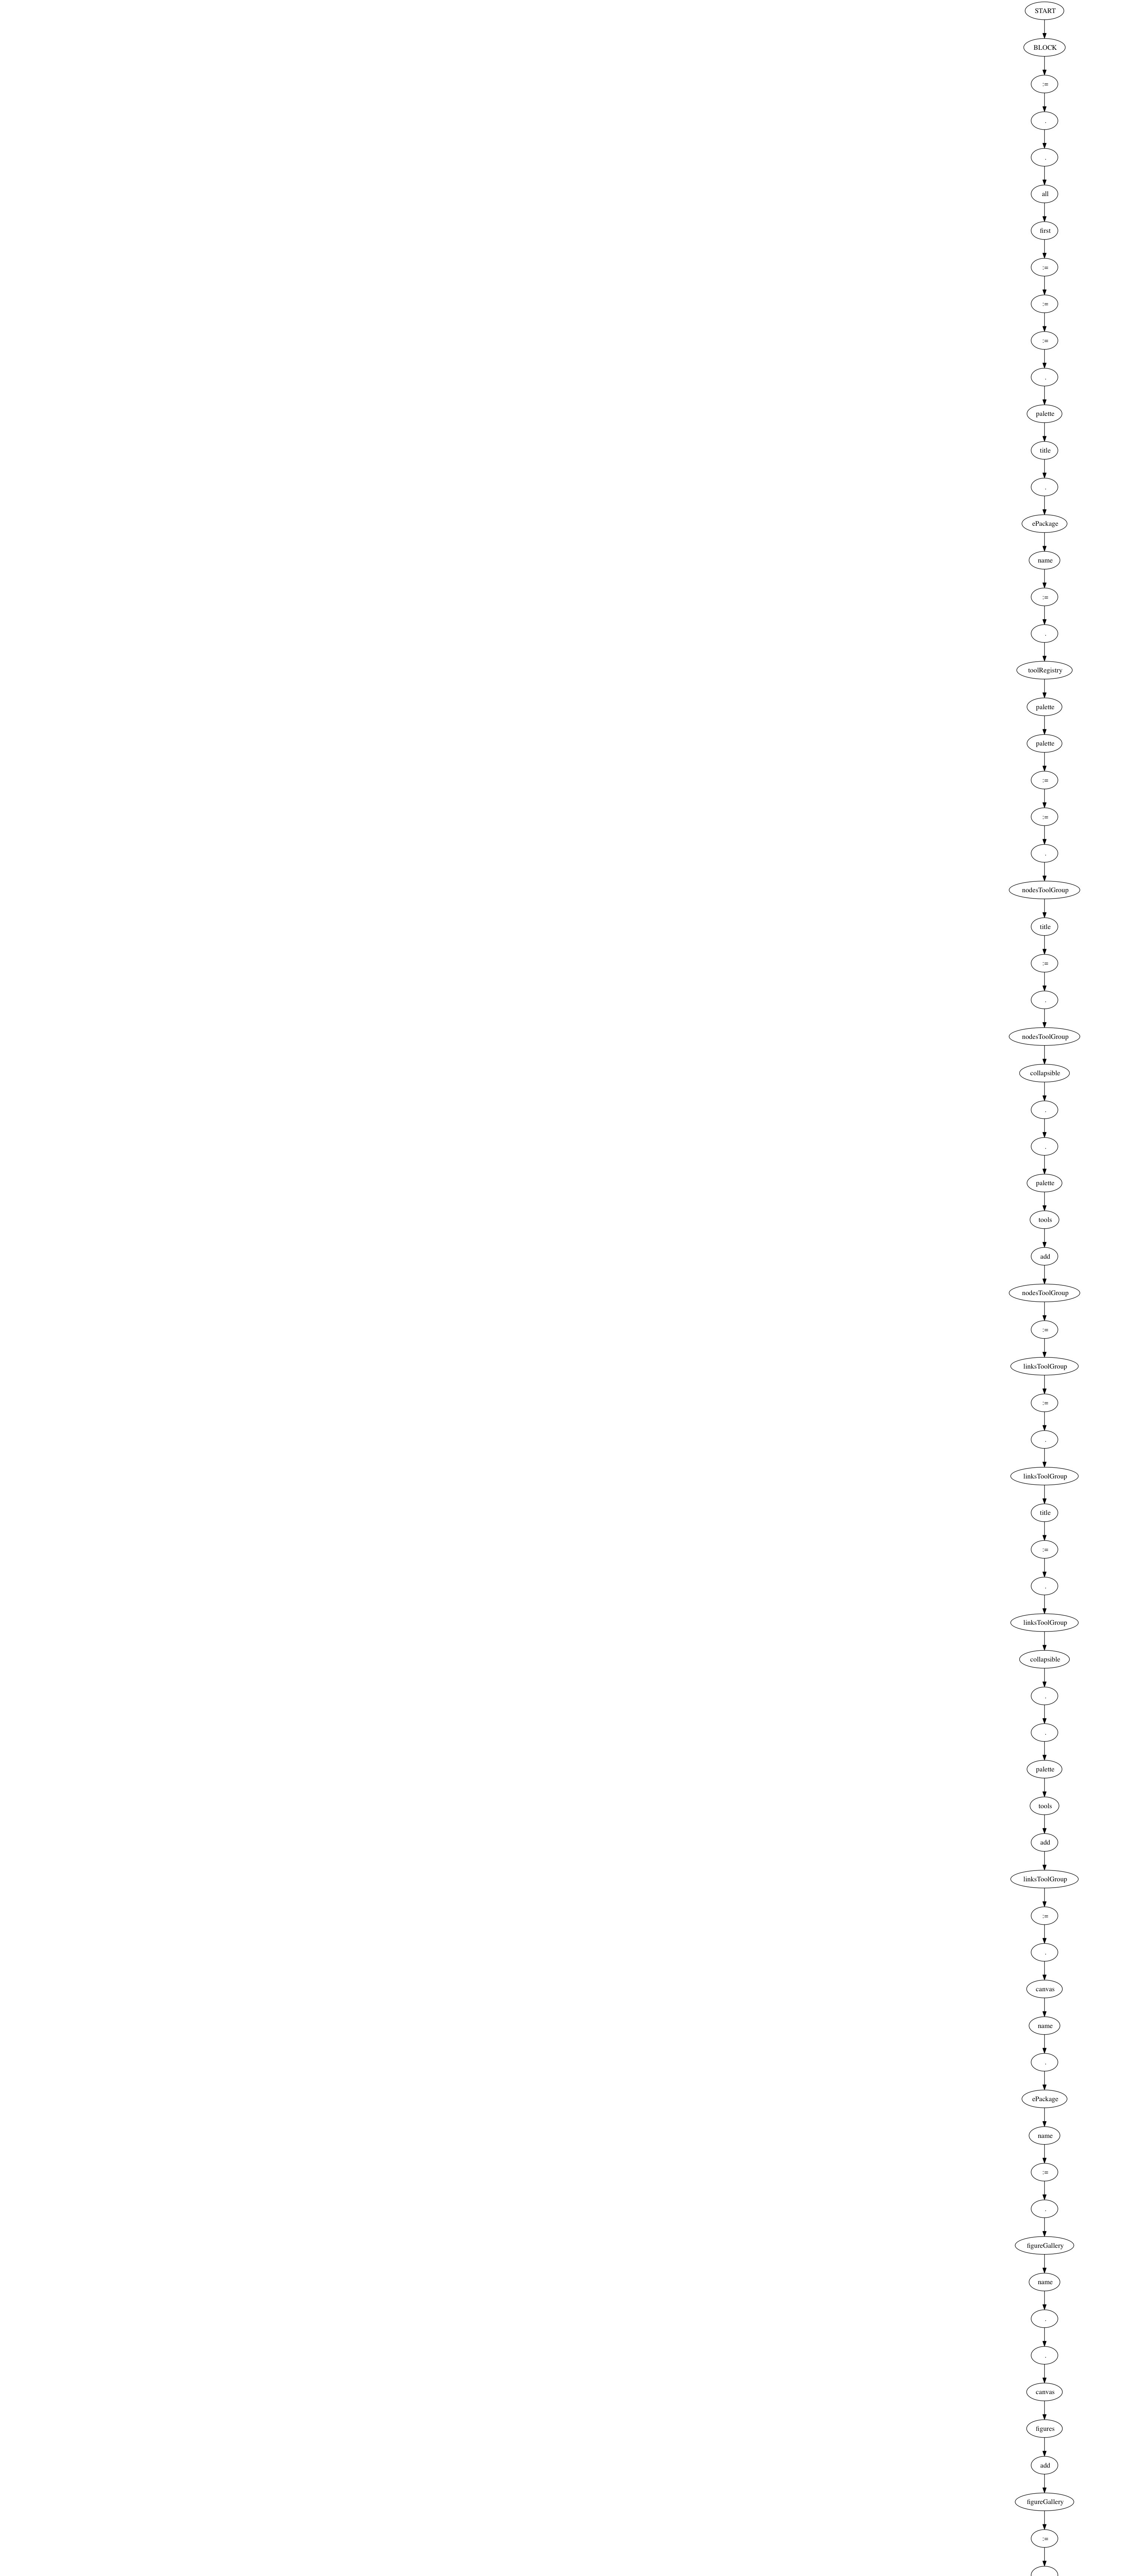
\includegraphics[height=0.97\textheight]{./figures/eug_1.png}
EuGENia Part 1
\end{minipage}
\begin{minipage}[b]{\textwidth}
\centering
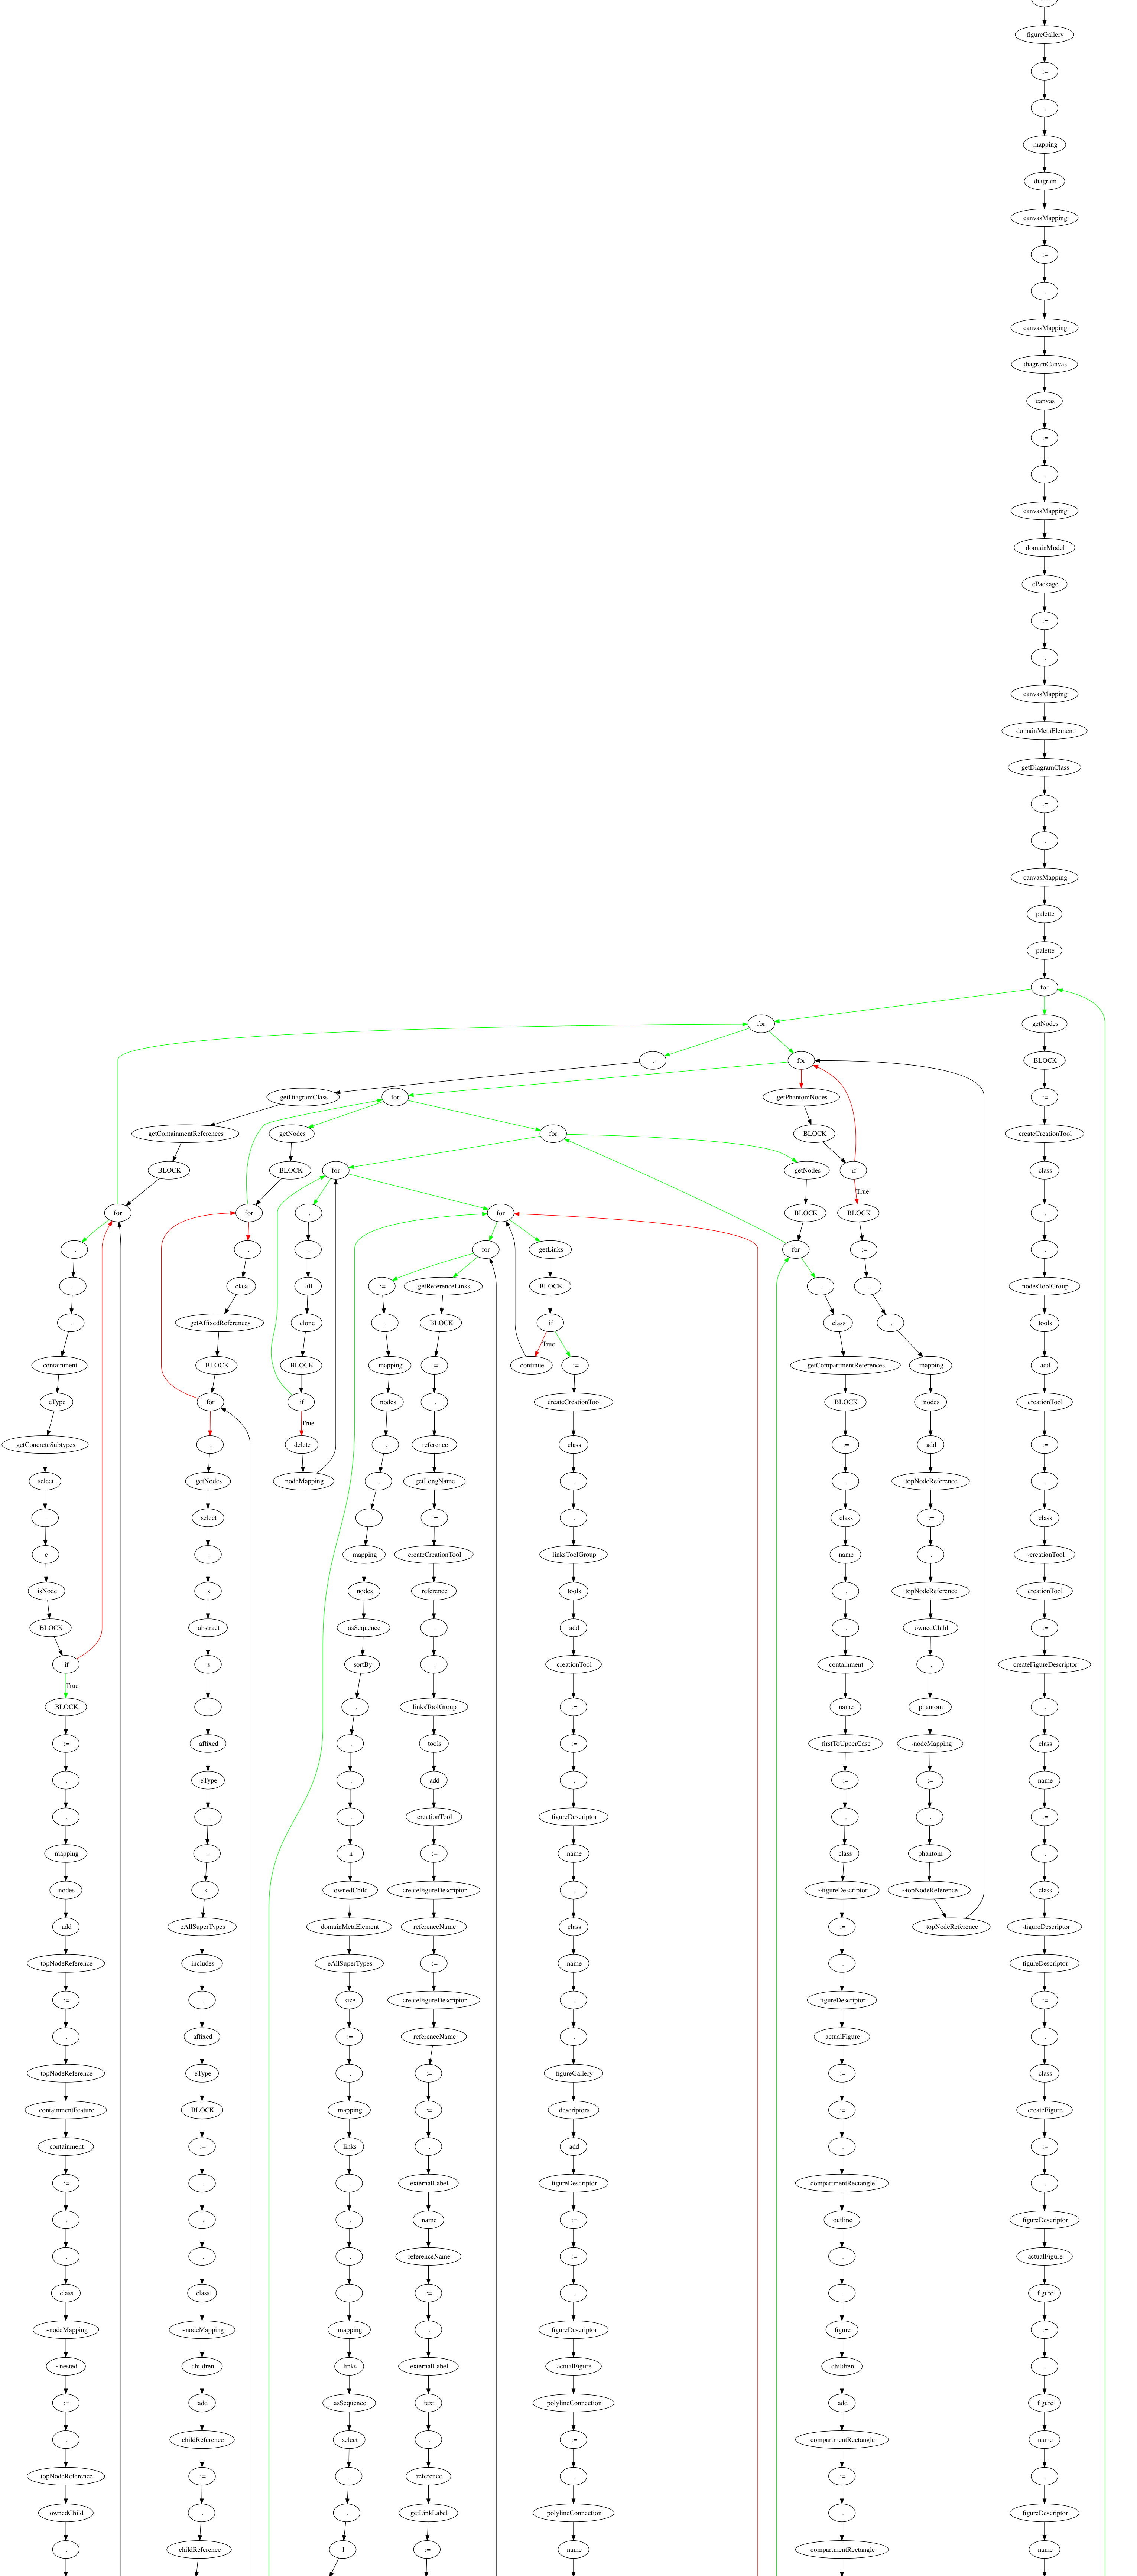
\includegraphics[height=0.97\textheight]{./figures/eug_2.png}
EuGENia Part 2
\end{minipage}
\begin{minipage}[b]{\textwidth}
\centering
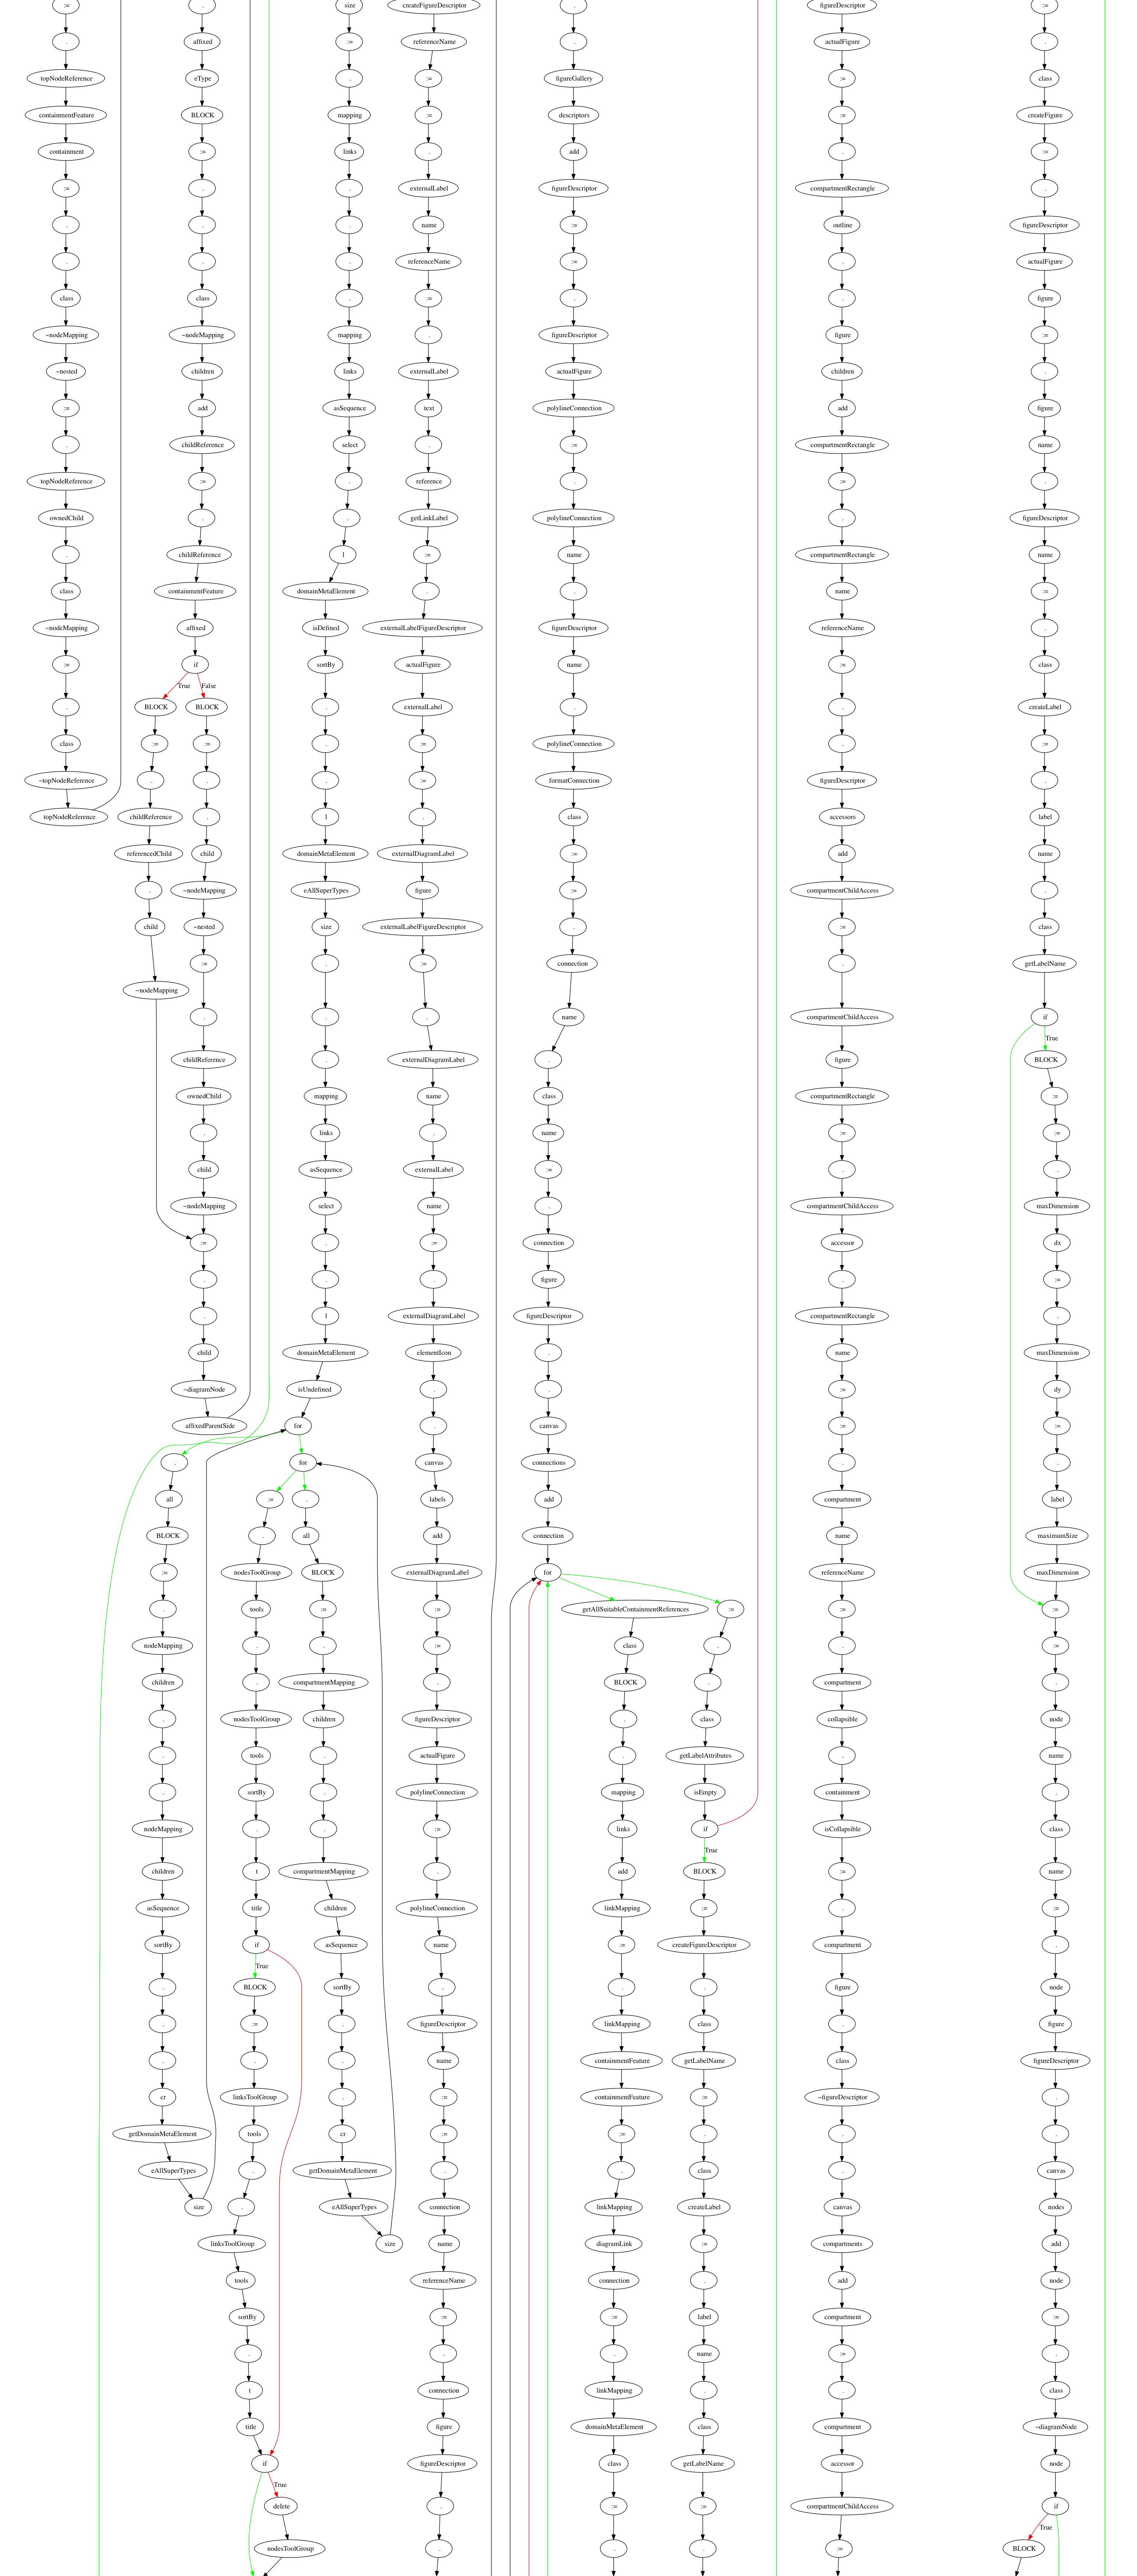
\includegraphics[height=0.97\textheight]{./figures/eug_3.png}
EuGENia Part 3
\end{minipage}
\begin{minipage}[b]{\textwidth}
\centering
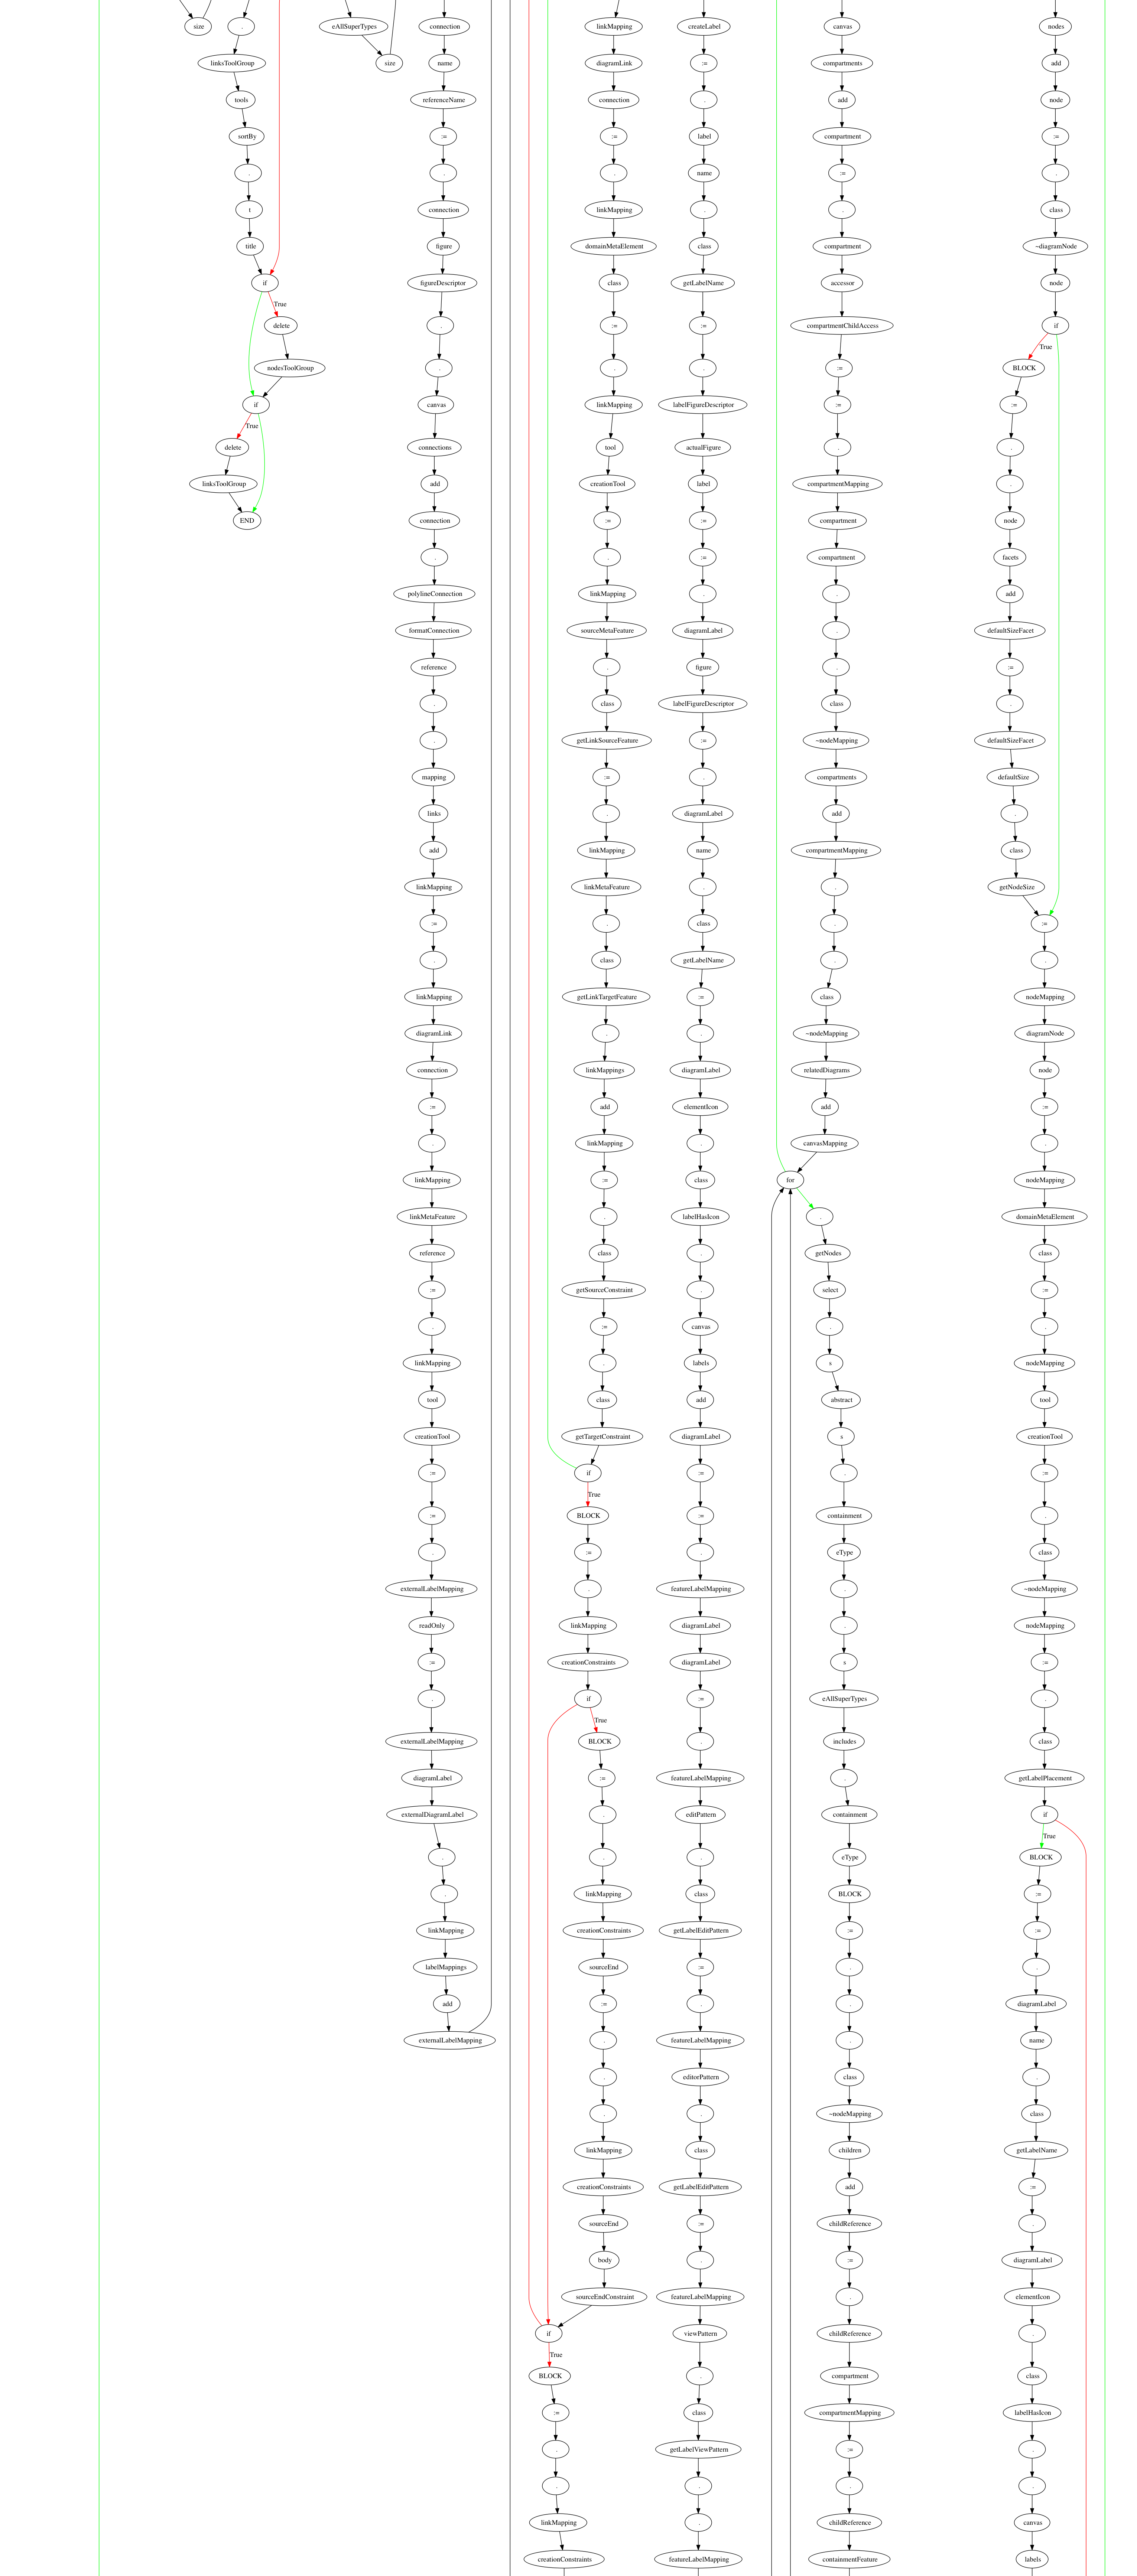
\includegraphics[height=0.97\textheight]{./figures/eug_4.png}
EuGENia Part 4
\end{minipage}
\begin{minipage}[b]{\textwidth}
\centering
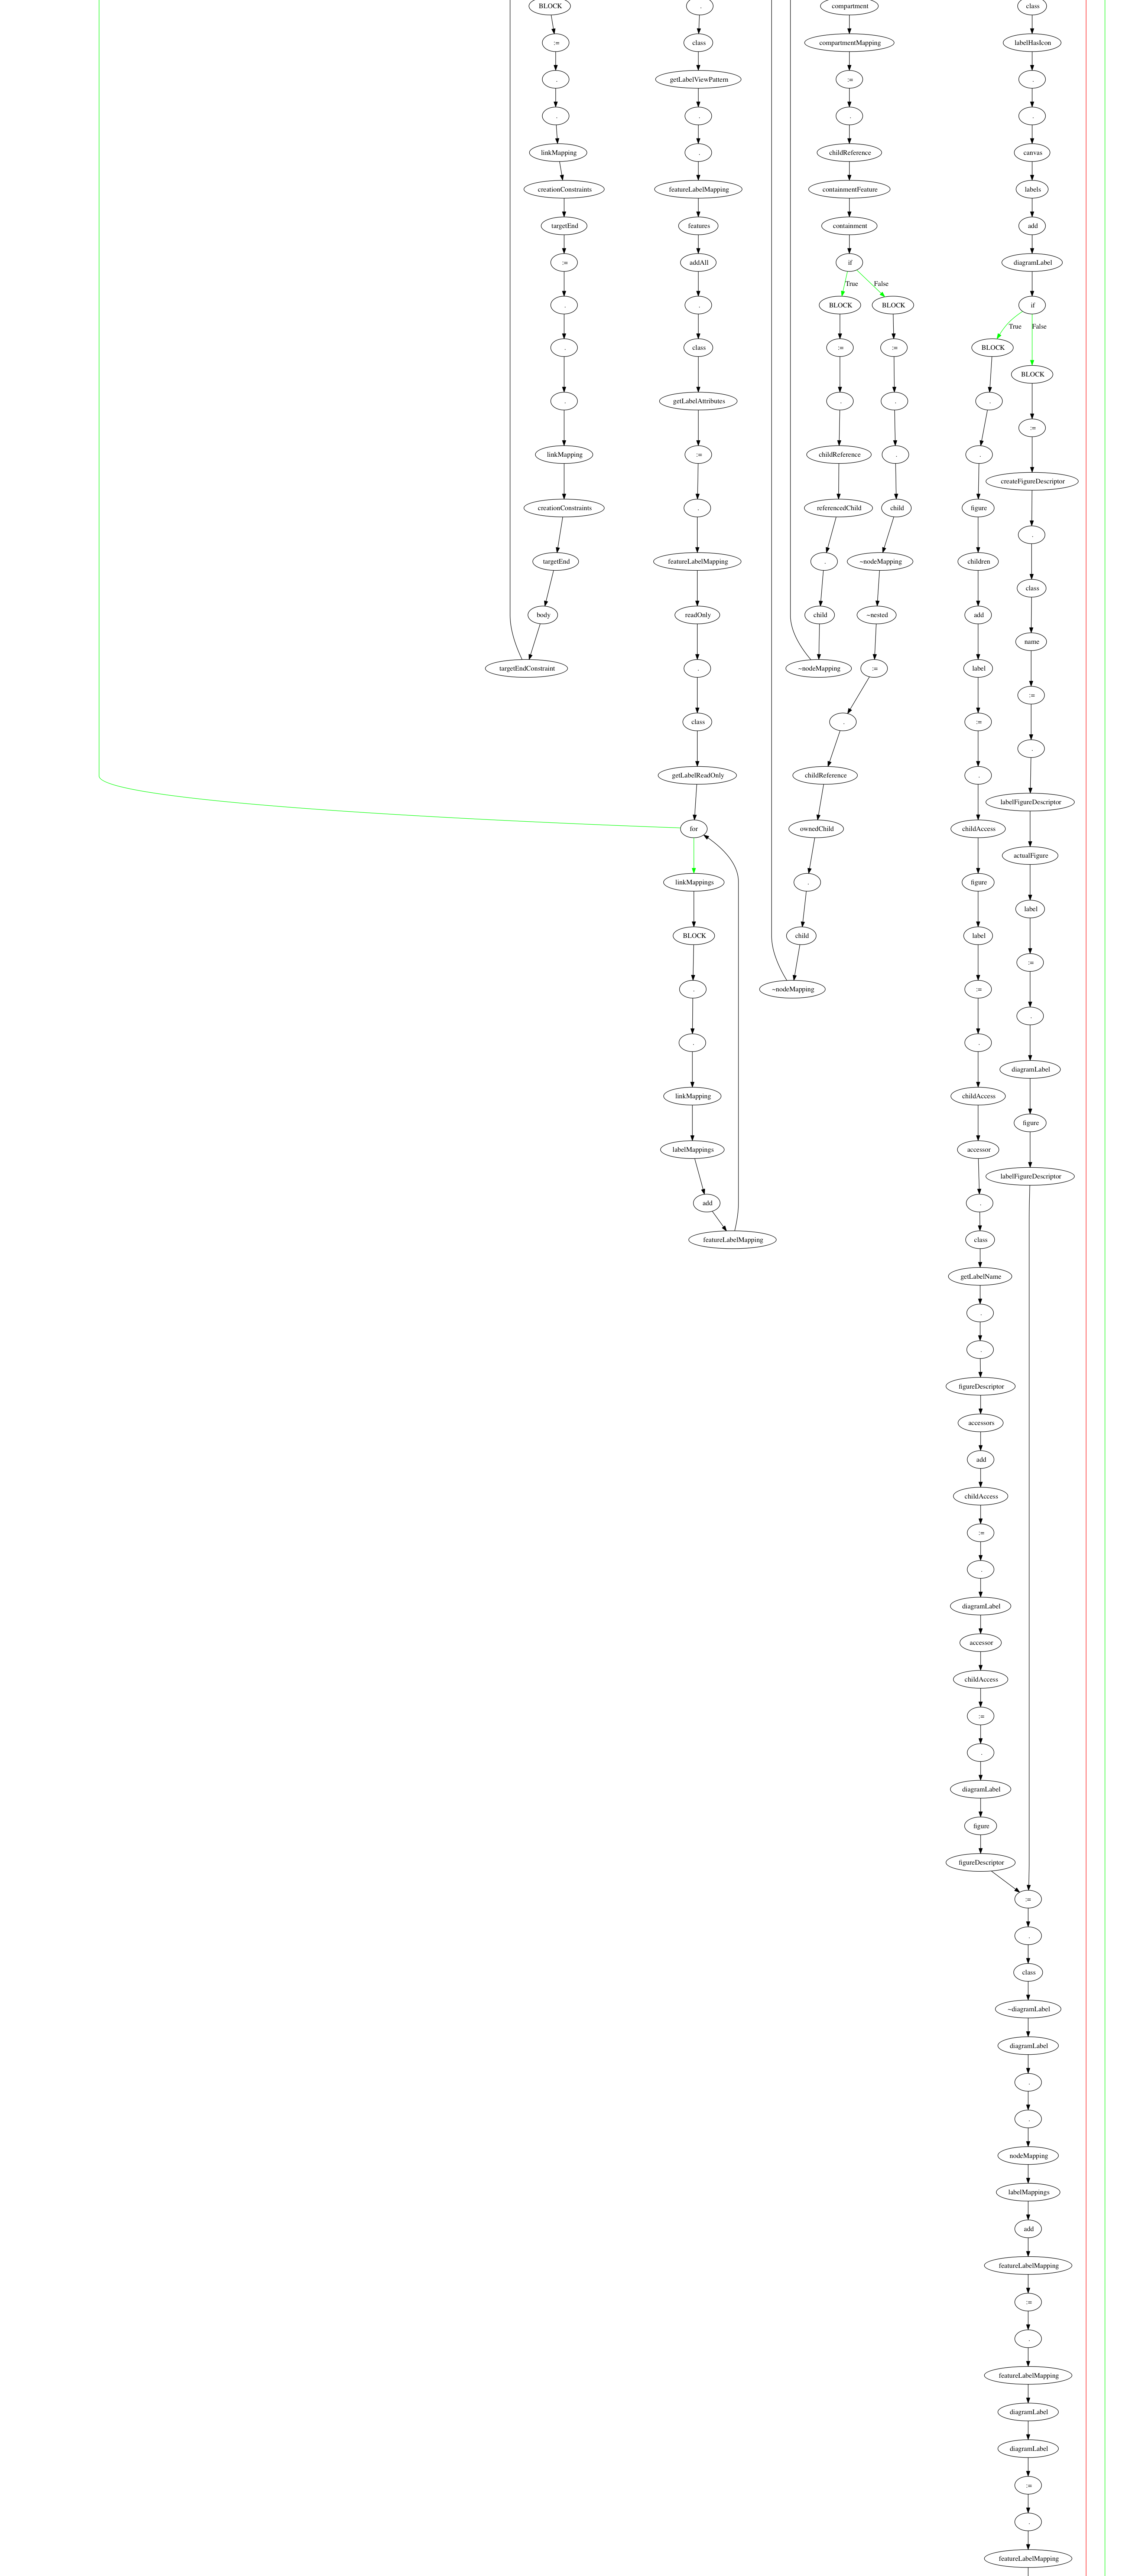
\includegraphics[height=0.97\textheight]{./figures/eug_5.png}
EuGENia Part 5
\end{minipage}
\begin{minipage}[b]{\textwidth}
\centering
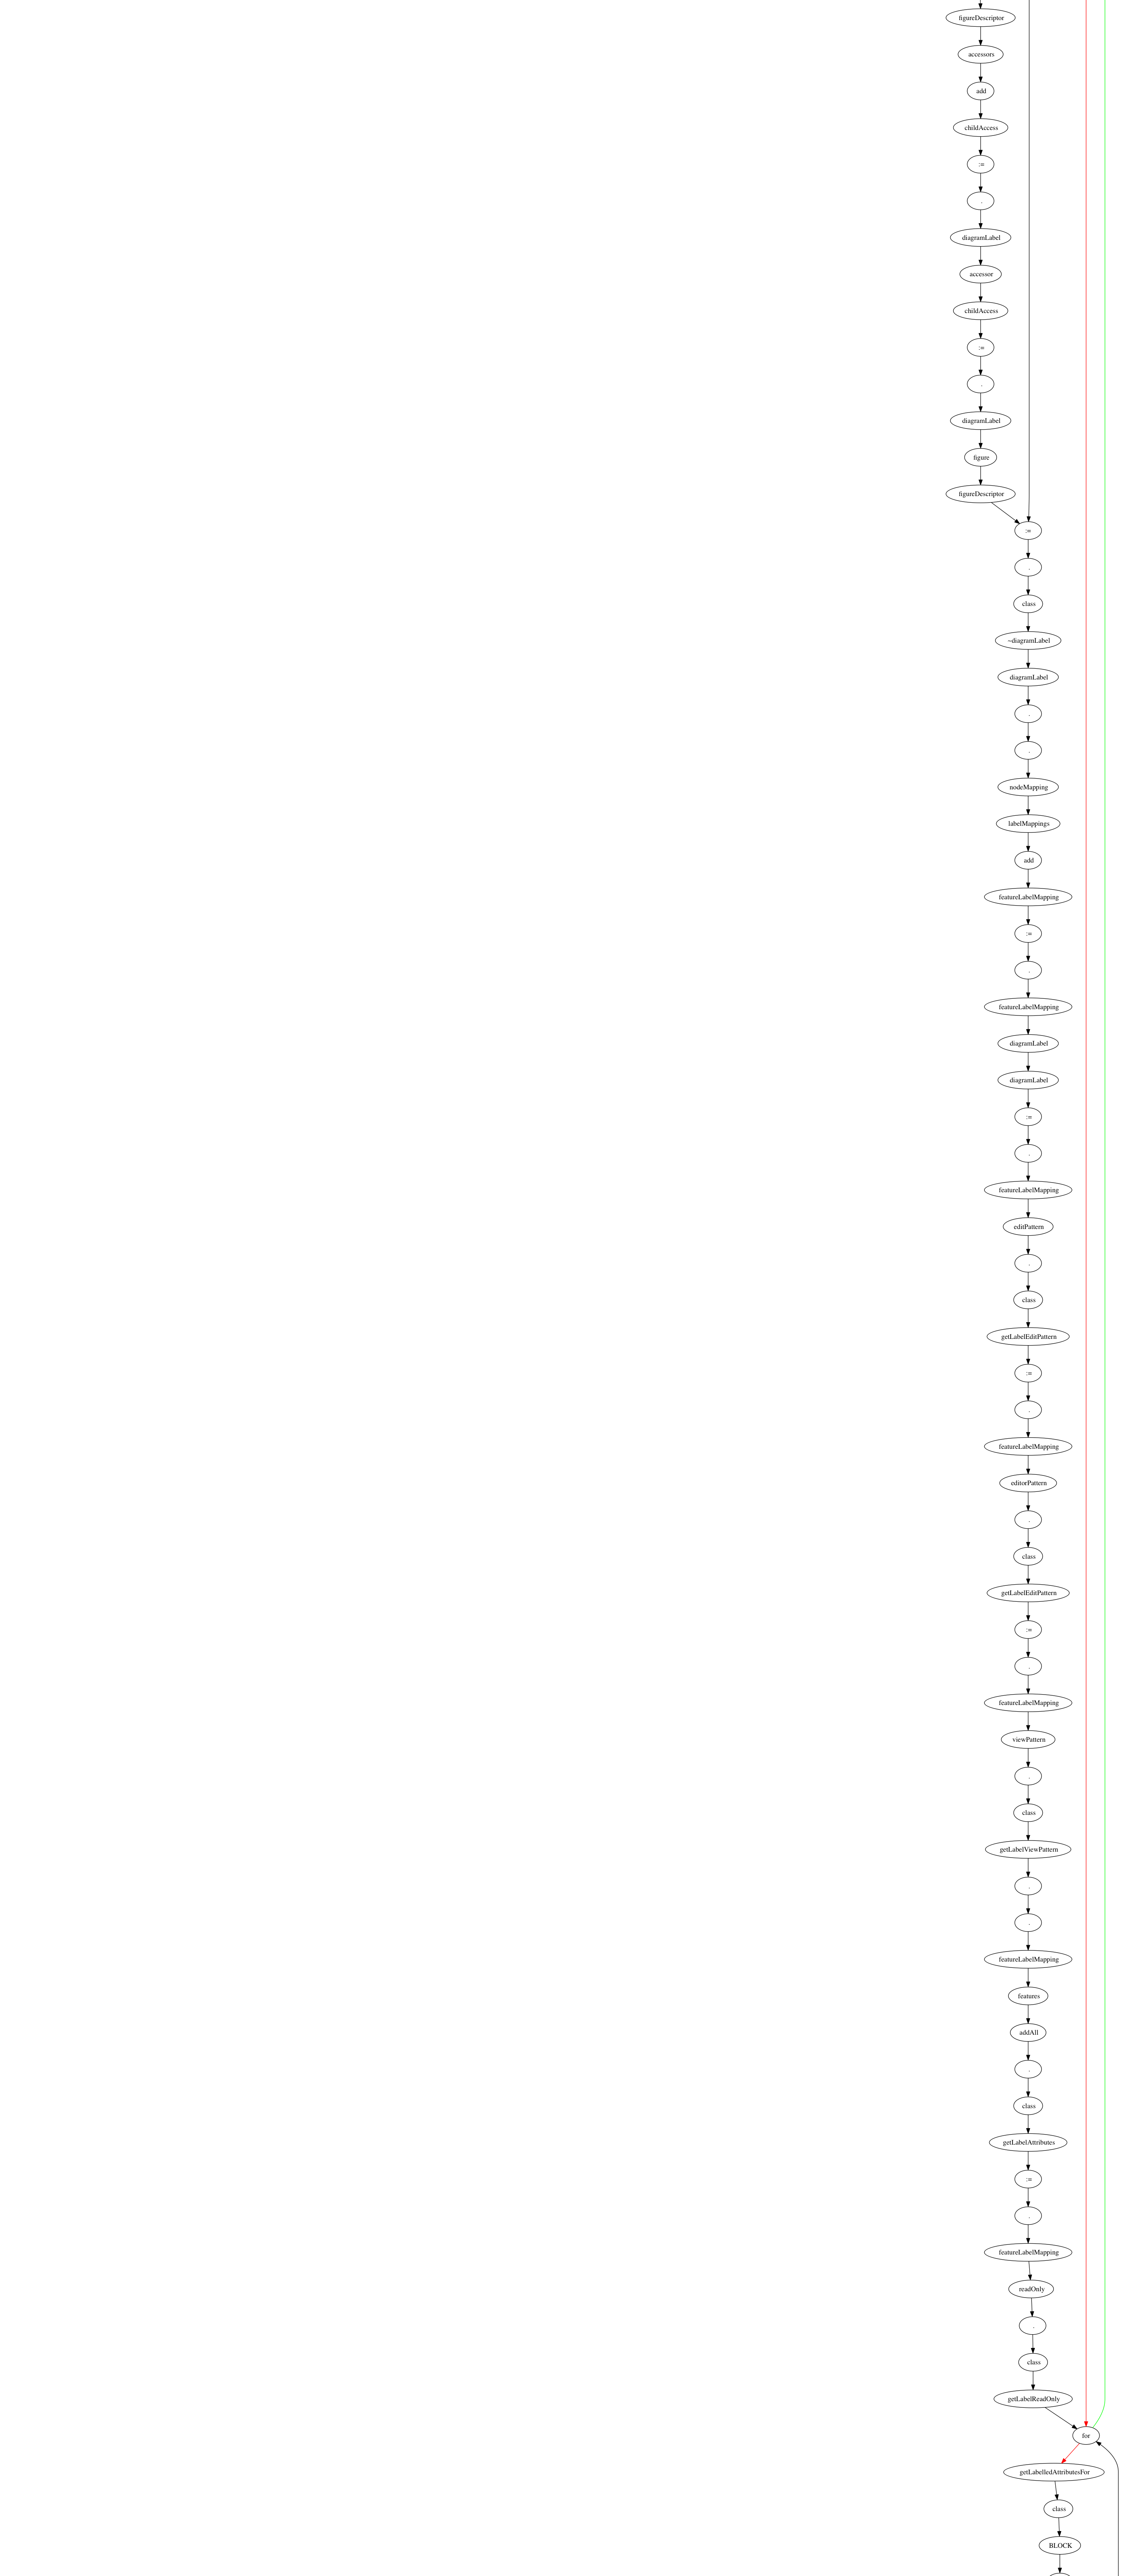
\includegraphics[height=0.97\textheight]{./figures/eug_6.png}
EuGENia Part 6
\end{minipage}
\begin{minipage}[b]{\textwidth}
\centering
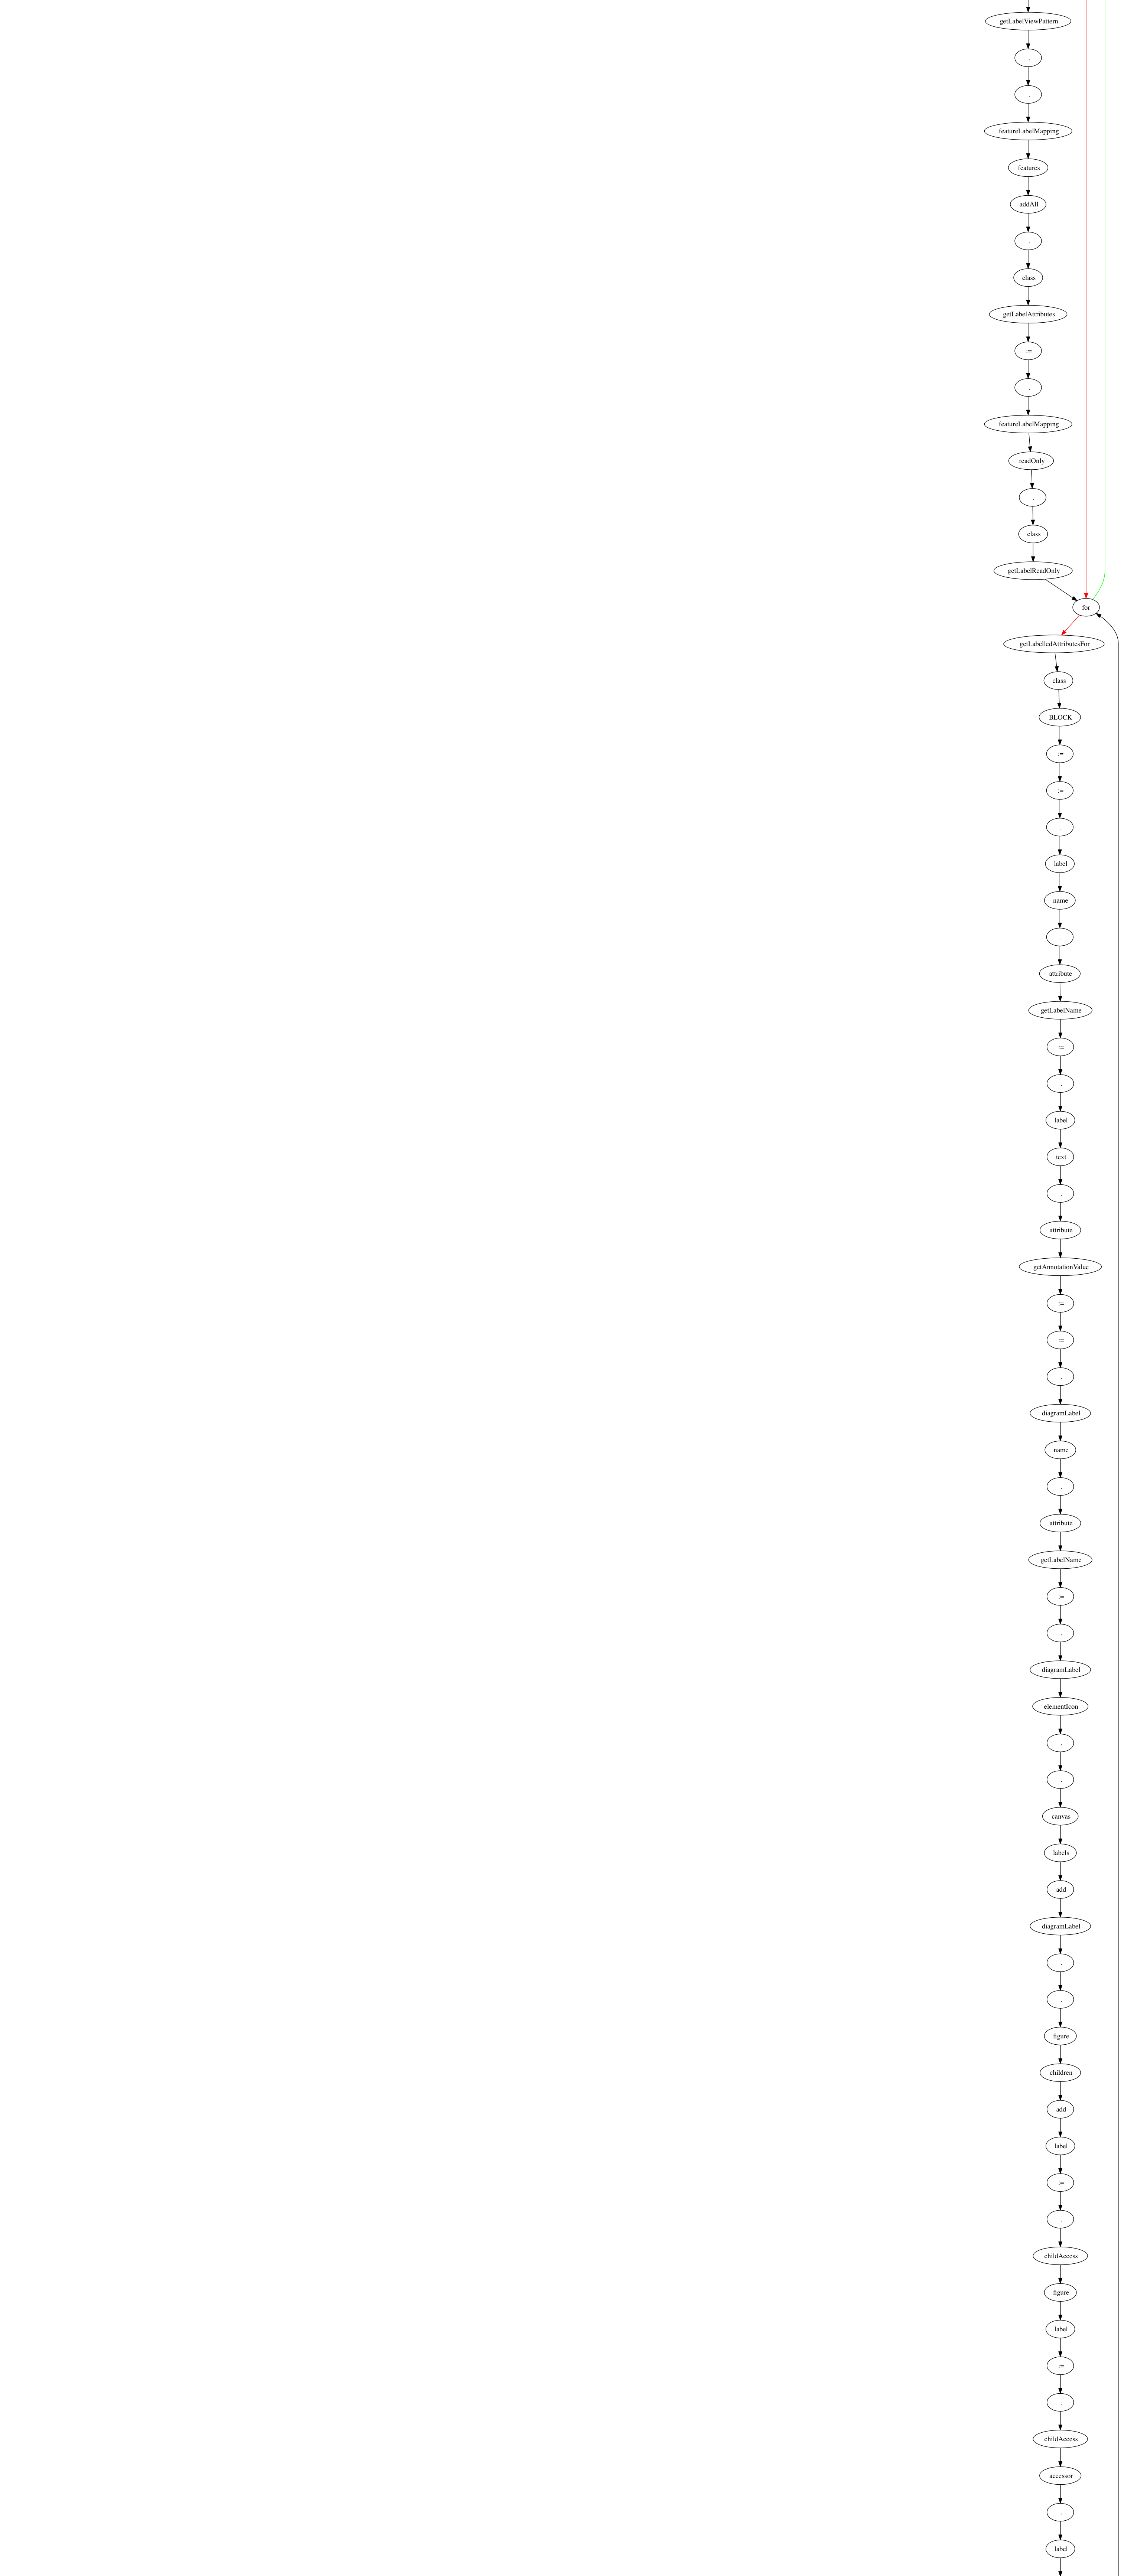
\includegraphics[height=0.97\textheight]{./figures/eug_7.png}
EuGENia Part 7
\end{minipage}
\begin{minipage}[b]{\textwidth}
\centering
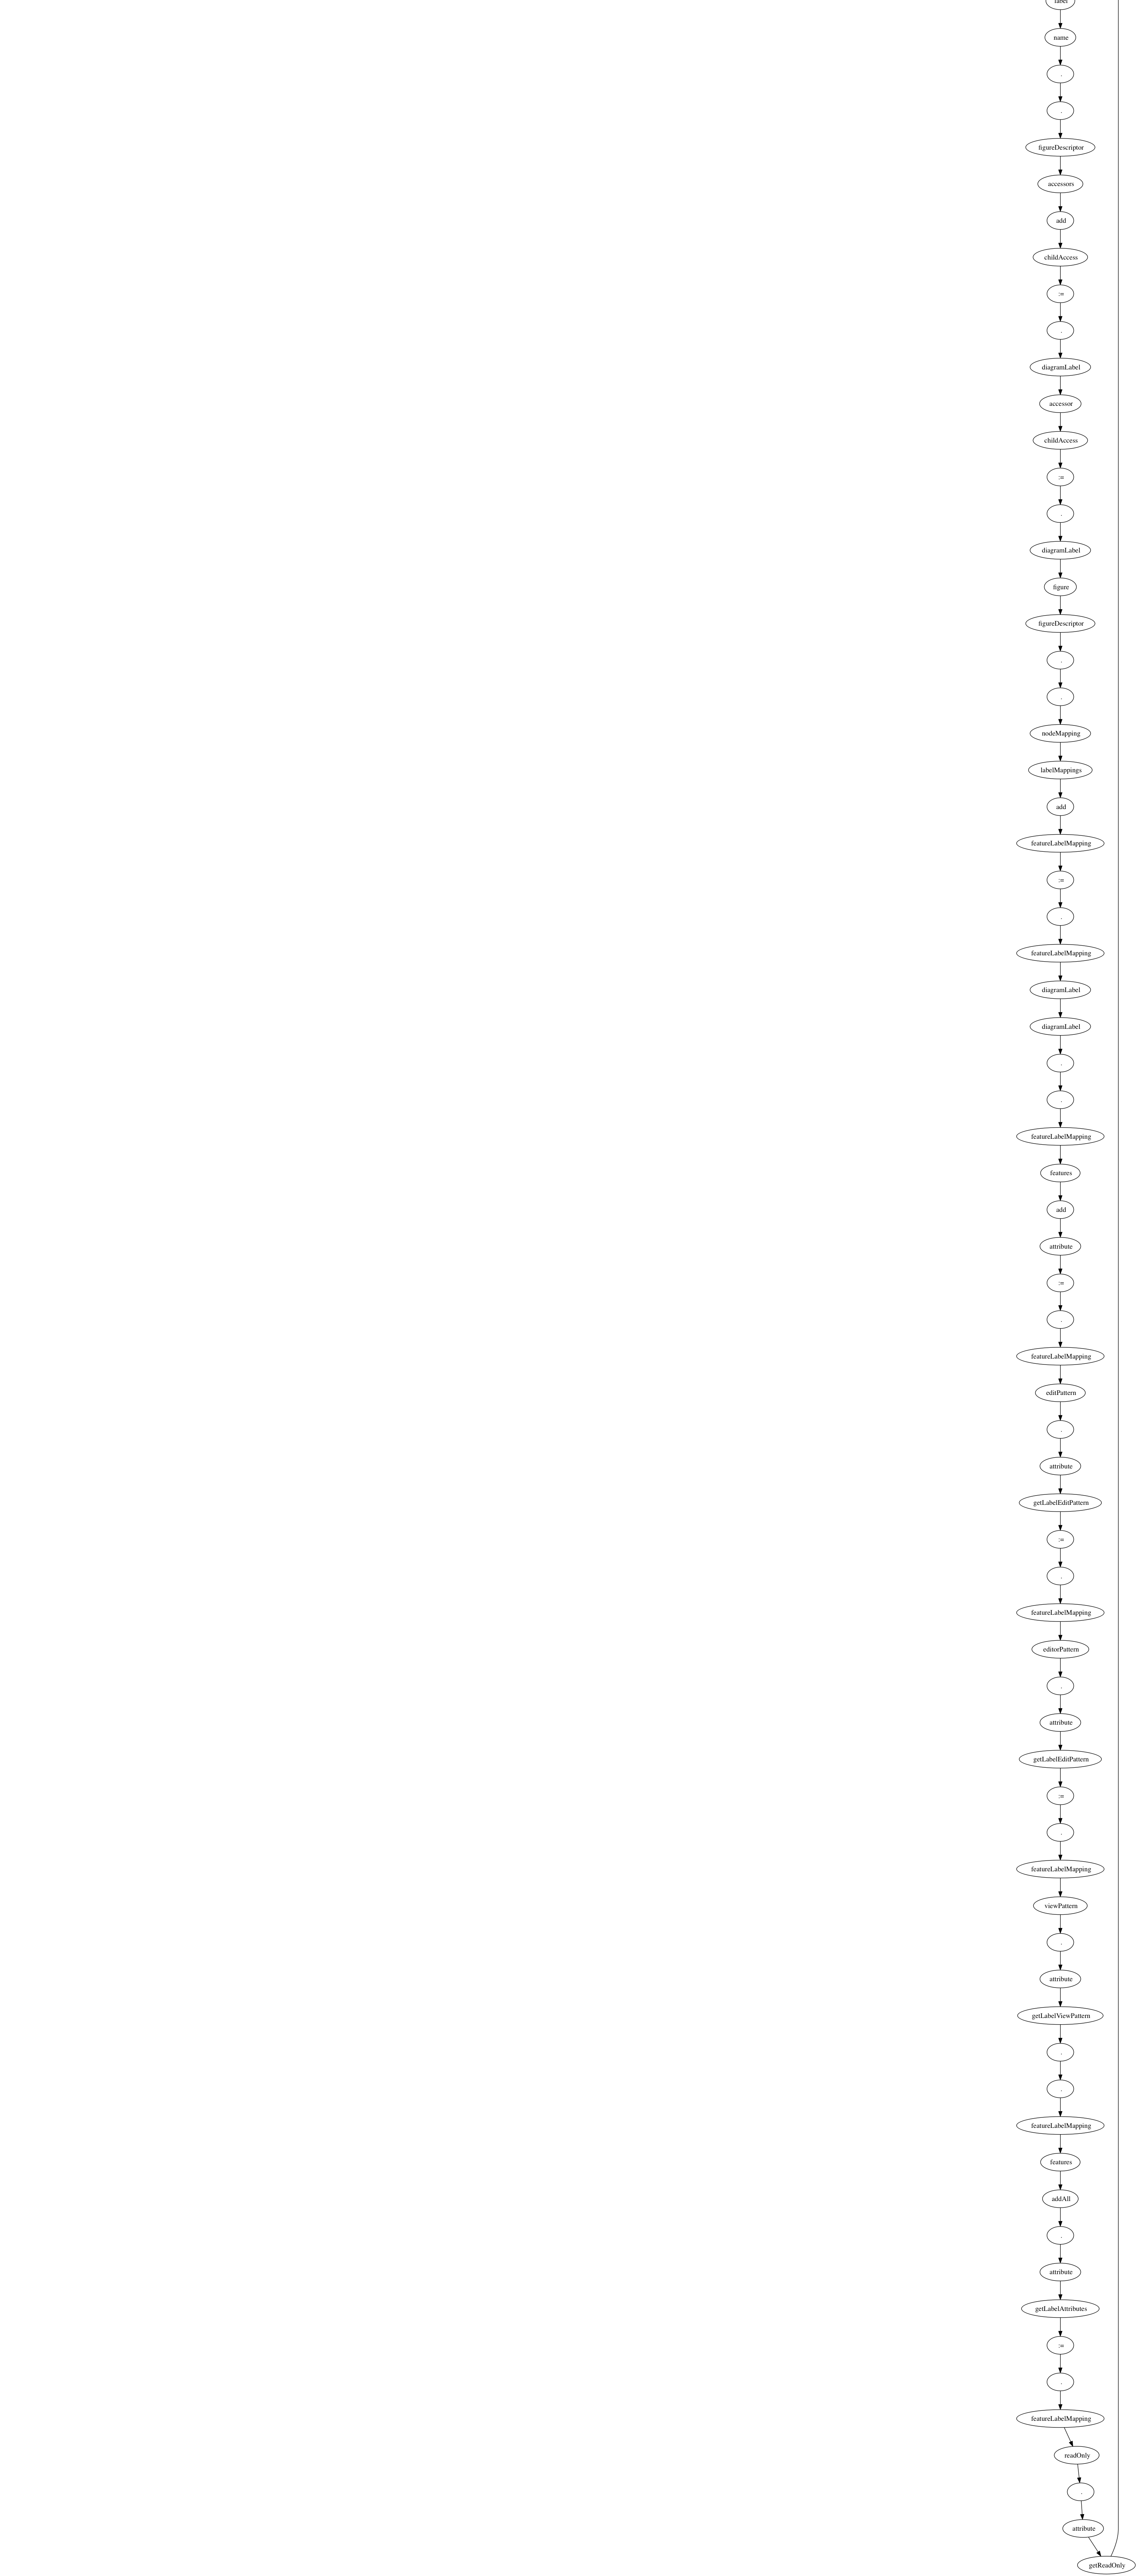
\includegraphics[height=0.97\textheight]{./figures/eug_9.png}
EuGENia Part 8
\end{minipage}
